\documentclass{beamer}
\usepackage[utf8]{inputenc}
\usepackage[spanish]{babel}
\usepackage{graphicx}
\usepackage{subfigure}
\usepackage{algorithm}
\usepackage{algpseudocode}
\usepackage{amsmath}
\usepackage{amsfonts}
\usepackage{amssymb}
 \usetheme{Warsaw}
\title{Generalized mean for robust principal component analysis}
\author{Erick S. Alvarez Valencia}
\begin{document}
\begin{frame}
	\maketitle
	\begin{block}{Autores del paper}
		Jiyong Oh, Nojun Kwak
	\end{block}
\end{frame}

\begin{frame}{Contenido}
	\begin{enumerate}
		\item Algoritmo clásico: PCA.
		\item Media muestral usando la media generalizada.
		\item Versión robusta de PCA usando la media generalida.
		\item Experimentos realizados
		\begin{enumerate}
			\item Experimento con la media generalizada.
			\item Experimentos con PCA robusto.
		\end{enumerate}
		\item Conclusiones.
	\end{enumerate}
\end{frame}

\begin{frame}{Algoritmo clásico: PCA}
	\begin{block}{Motivación}
		Se tiene un conjunto de $m$ datos $X = (X_1, X_2, ..., X_m)$ los cuales viven en $R^n$ y con matriz de covarianza $\Sigma$.\\~\\
		
		Suponiendo media cero para dicho conjunto de datos, se busca una matriz $W \in R^{nxm}$ con $m < n$ tal que al realizar la proyección $W^T X$ se preserve la máxima cantidad de variabilidad en la misma.
	\end{block}
\end{frame}

\begin{frame}{Algoritmo clásico: PCA}
	Sea $Y = (Y_1, Y_2, ..., Y_m)$ donde $Y_i = W^T X_i$ las proyecciones del conjunto de datos con respecto a la matriz $W$. El problema de optimización se define como:
	
	\begin{align}
	\label{eqn:eqlabel}
	\begin{split}
	\underset{W}{\text{arg max}}\ tr(W^T \Sigma W)\\
		s.a.\ W^T W = I
	\end{split}
	\end{align}
	
	Donde $\Sigma = \frac{1}{m} \sum_{i = 1}^m X_i X_i^T$. Lo anterior es equivalente a
	
	\begin{align}
	\label{eqn:eqlabel}
	\begin{split}
		J_{L_2}(W) = \frac{1}{m} \sum_{i = 1}^m ||X_i - W W^T X_i||_2^2
	\end{split}
	\end{align}
\end{frame}

\begin{frame}{Algoritmo clásico: PCA}
	Se puede mostrar que la solución del problema de optimización anterior es igual a
	
	\begin{align}
	\label{eqn:eqlabel}
	\begin{split}
			\Sigma v = \lambda v
	\end{split}
	\end{align}
	
	Donde $v$ es el eigenvector asociado al eigenvalor más grande de la matriz de covarianza. ¡Los eigenvalores explican la variabilidad!
\end{frame}

\begin{frame}{Algoritmo clásico: PCA}
	Aunque PCA es muy simple y un buen método de reducción de dimensión, cuenta con fallos y uno de ellos es el hecho de que es sensible ante datos atípicos. El problema recae al hecho de que estos datos generan una gran variabilidad en el conjunto de datosy PCA puede dar soluciones no deseadas, y esto ocurre porque la función de optimización está formulada en base el error cuadrático medio y este a su vez usa la norma $L_2$.
\end{frame}

\begin{frame}{Media generalizada}
	La media generalizada se define como:
	
	\begin{block}{Definición GM}
		Sea $p \neq 0$ y sea $A = (a_1, a_2, ..., a_m)^T$ un conjunto de datos positivos.
		\begin{align}
		\label{eqn:eqlabel}
		\begin{split}
			M_p\{a_1, a_2, ..., a_m\} = (\frac{1}{m} \sum_{i = 1}^m a_i^p)^{1/p}
		\end{split}
		\end{align}
	\end{block}
	
	Casos especiales:
	\begin{enumerate}
		\item Si $p = 1$ se tiene la media aritmética.
		\item Si $p \rightarrow 0$ se tiene la media geométrica.
		\item Si $p = -1$ se tiene la media armónica.
	\end{enumerate}
\end{frame}

\begin{frame}{Media generalizada}
	Se puede demostrar que:
	
	\begin{align}
	\label{eqn:eqlabel}
	\begin{split}
		\sum_{i = 1}^m a_i^p = b_1 a_1 + b_2 a_2 + ... + b_m a_m
	\end{split}
	\end{align}
	
	Donde $b_i = a_i^{p - 1},\ i = 1, 2, ..., m$.
\end{frame}

\begin{frame}{Media muestral usando GM}
	PCA asume que los datos tienen media cero. La media muestral se puede formar como un problema de mínimos cuadrados.
	
	\begin{align}
	\label{eqn:eqlabel}
	\begin{split}
		m_s = \underset{m}{\text{arg min}}\ \frac{1}{M} \sum_{i = 1}^M ||x_i - m||_2^2
	\end{split}
	\end{align}
	
	Como se usa la norma $L_2$ la media muestral es sensible ante datos atípicos.
\end{frame}

\begin{frame}{Media muestral usando GM}
	Propuesta: Usar GM en la función de costo anterior para obtener una versión más robusta.
	
	\begin{align}
	\label{eqn:eqlabel}
	\begin{split}
		m_g = \underset{m}{\text{arg min}}\ (\frac{1}{M} \sum_{i = 1}^M (||x_i - m||_2^2)^p)^{1/p},\ p > 0
	\end{split}
	\end{align}
	
	Como $p > 0$ lo anterior es igual a
	
	\begin{align}
	\label{eqn:eqlabel}
	\begin{split}
		m_g = \underset{m}{\text{arg min}}\ \sum_{i = 1}^M (||x_i - m||_2^2)^p
	\end{split}
	\end{align}
\end{frame}

\begin{frame}{Media muestral usando GM}
	Podemos utilizar la descomposición de GM como combinación lineal
	
	\begin{align}
	\label{eqn:eqlabel}
	\begin{split}
	\sum_{i = 1}^M (||x_i - m||_2^2)^p \approx \sum_{i = 1}^M \alpha_i^t ||x_i - m||_2^2
	\end{split}
	\end{align}
	
	Donde $\alpha_i^t = (||x_i - m^t||_2^2)^{p - 1}$. Para la ecuación anterior la aproximación se convertiría en igualdad cuando $m = m^t$. El siguiente paso es encontrar $m^{t + 1}$ tal que minimice $\alpha^t$ y en esta caso se puede derivar e igualar a cero, y con un poco de álgebra se obtiene:
	
	\begin{align}
	\label{eqn:eqlabel}
	\begin{split}
		m^{t + 1} = \frac{1}{\sum_{j = 1}^M \alpha_j^t} \sum_{i = 1}^M \alpha_i^t x_i
	\end{split}
	\end{align}
	
	Con esto se propone un método de optimización basado en el algoritmo EM.
\end{frame}

\begin{frame}{Media muestral usando GM}
	\begin{algorithm}[H]
		\caption{Media generalizada}
		\begin{algorithmic}[1]
			\Procedure{GeneralizedMean}{$X$, $p$}
			\State t $\gets$ 0.
			\State $m^t$ $\gets$ $m_s$.
			\While{No convergencia}
			\State $\textbf{Aproximación}:$ Calcular $\alpha_1^t, \alpha_2^t, ..., \alpha_m^t$ usando (9).
			\State $\textbf{Minimización}:$ Usando las alfas calculadas en el paso anterior, calcular $m^{t + 1}$ con (10).
			\State t $\gets$ t + 1.
			\EndWhile
			\State \textbf{return} $m_g = m^t$.
			\EndProcedure
		\end{algorithmic}
	\end{algorithm}
\end{frame}

\begin{frame}{PCA robusto usando GM}
	Retomando PCA, tenemos que el error de reconstrucción generado por las proyecciones se calcula como
	
	\begin{align}
	\label{eqn:eqlabel}
	\begin{split}
		e(W) = \hat{X}^T \hat{X} - \hat{X}^T W W^T \hat{X}
	\end{split}
	\end{align}
	
	Donde $\hat{X} = X - m$, es decir, los datos contienen media cero. Podemos aplicar en concepto de media generalida a la ecuación anterior para definir el nuevo problema de optimización, obteniendo:
	
	\begin{align}
	\label{eqn:eqlabel}
	\begin{split}
		W_g = \underset{W^T W = 1}{\text{arg min}}\ (\frac{1}{M} \sum_{i = 1}^M [e_i(W)]^p)^{1 / p},\ p > 0
	\end{split}
	\end{align}
	
	Como $p > 0$ lo anterior es equivalente al siguiente problema
	
	\begin{align}
	\label{eqn:eqlabel}
	\begin{split}
		W_g = \underset{W^T W = 1}{\text{arg min}}\ \sum_{i = 1}^M [e_i(W)]^p,
	\end{split}
	\end{align}
\end{frame}

\begin{frame}{PCA robusto usando GM}
	Aplicando la descomposición de la media generalizada mostrada anteriormente tenemos
	
	\begin{align}
	\label{eqn:eqlabel}
	\begin{split}
		\sum_{i = 1}^M e_i(W)^p \approx \sum_{i = 1}^M \beta_i^t e_i(W)^p
	\end{split}
	\end{align}
	
	Donde $\beta_i^t = [e_i(W^t)]^{p - 1}$. Esta aproximación se vuelve exacta cuando $W = W^t$. Ahora para calcular $W^{t + 1}$ podemos usar la otra versión de la función objetivo de PCA
	
	\begin{align}
	\label{eqn:eqlabel}
	\begin{split}
		W^{t + 1} = \underset{W}{\text{arg max}}\ tr(W^T \Sigma_\beta^t W)\\
	s.a.\ W^T W = I
	\end{split}
	\end{align}
	
	Donde $\Sigma_\beta^t = \sum_{i = 1}^m \beta_i^t \hat{x_i} \hat{x_i}^T$.
\end{frame}

\begin{frame}{PCA robusto usando GM}
	\begin{algorithm}[H]
		\caption{PCA robusto con media generalizada}
		\begin{algorithmic}[1]
			\Procedure{RobustPCA}{$X$, $m_g$, $m$, $p$}
			\State t $\gets$ 0.
			\State $\hat{X} \gets X - m_g$.
			\State $W^t$ $\gets$ $W_{PCA}$.
			\While{No convergencia}
			\State $\textbf{Aproximación}:$ Fijando $W^t$, calcular $\beta_1^t, \beta_2^t, ..., \beta_m^t$ usando la ecuación (14).
			\State $\textbf{Optimización}:$ Usando las betas calculadas en el paso anterior, calcular $W^{t + 1}$ resolviendo el problema de eigenvalores-eigenvectores descrito en (15).
			\State t $\gets$ t + 1.
			\EndWhile
			\State \textbf{return} $W_g = W^t$.
			\EndProcedure
		\end{algorithmic}
	\end{algorithm}
\end{frame}

\begin{frame}{Experimento 1}
	Se generaron 100 datos de una bivariada Gaussiana con media $\mu_i = (0, 0)^T$ y matriz de covarianza $\Sigma_i = diag(0.5, 0.5)$ y se añeadieron 10 puntos atípicos de la misma distribución con media $\mu_o = (5, 5)^T$ y matriz de covarianza $\Sigma_o = diag(0.3, 0.3)^T$. Posteriorme se obtuvo la media muestral y la media generalizada con $p = 0.2$.
\end{frame}


\begin{frame}{Experimento 1}
	Resultados obtenidos
	\begin{figure}
		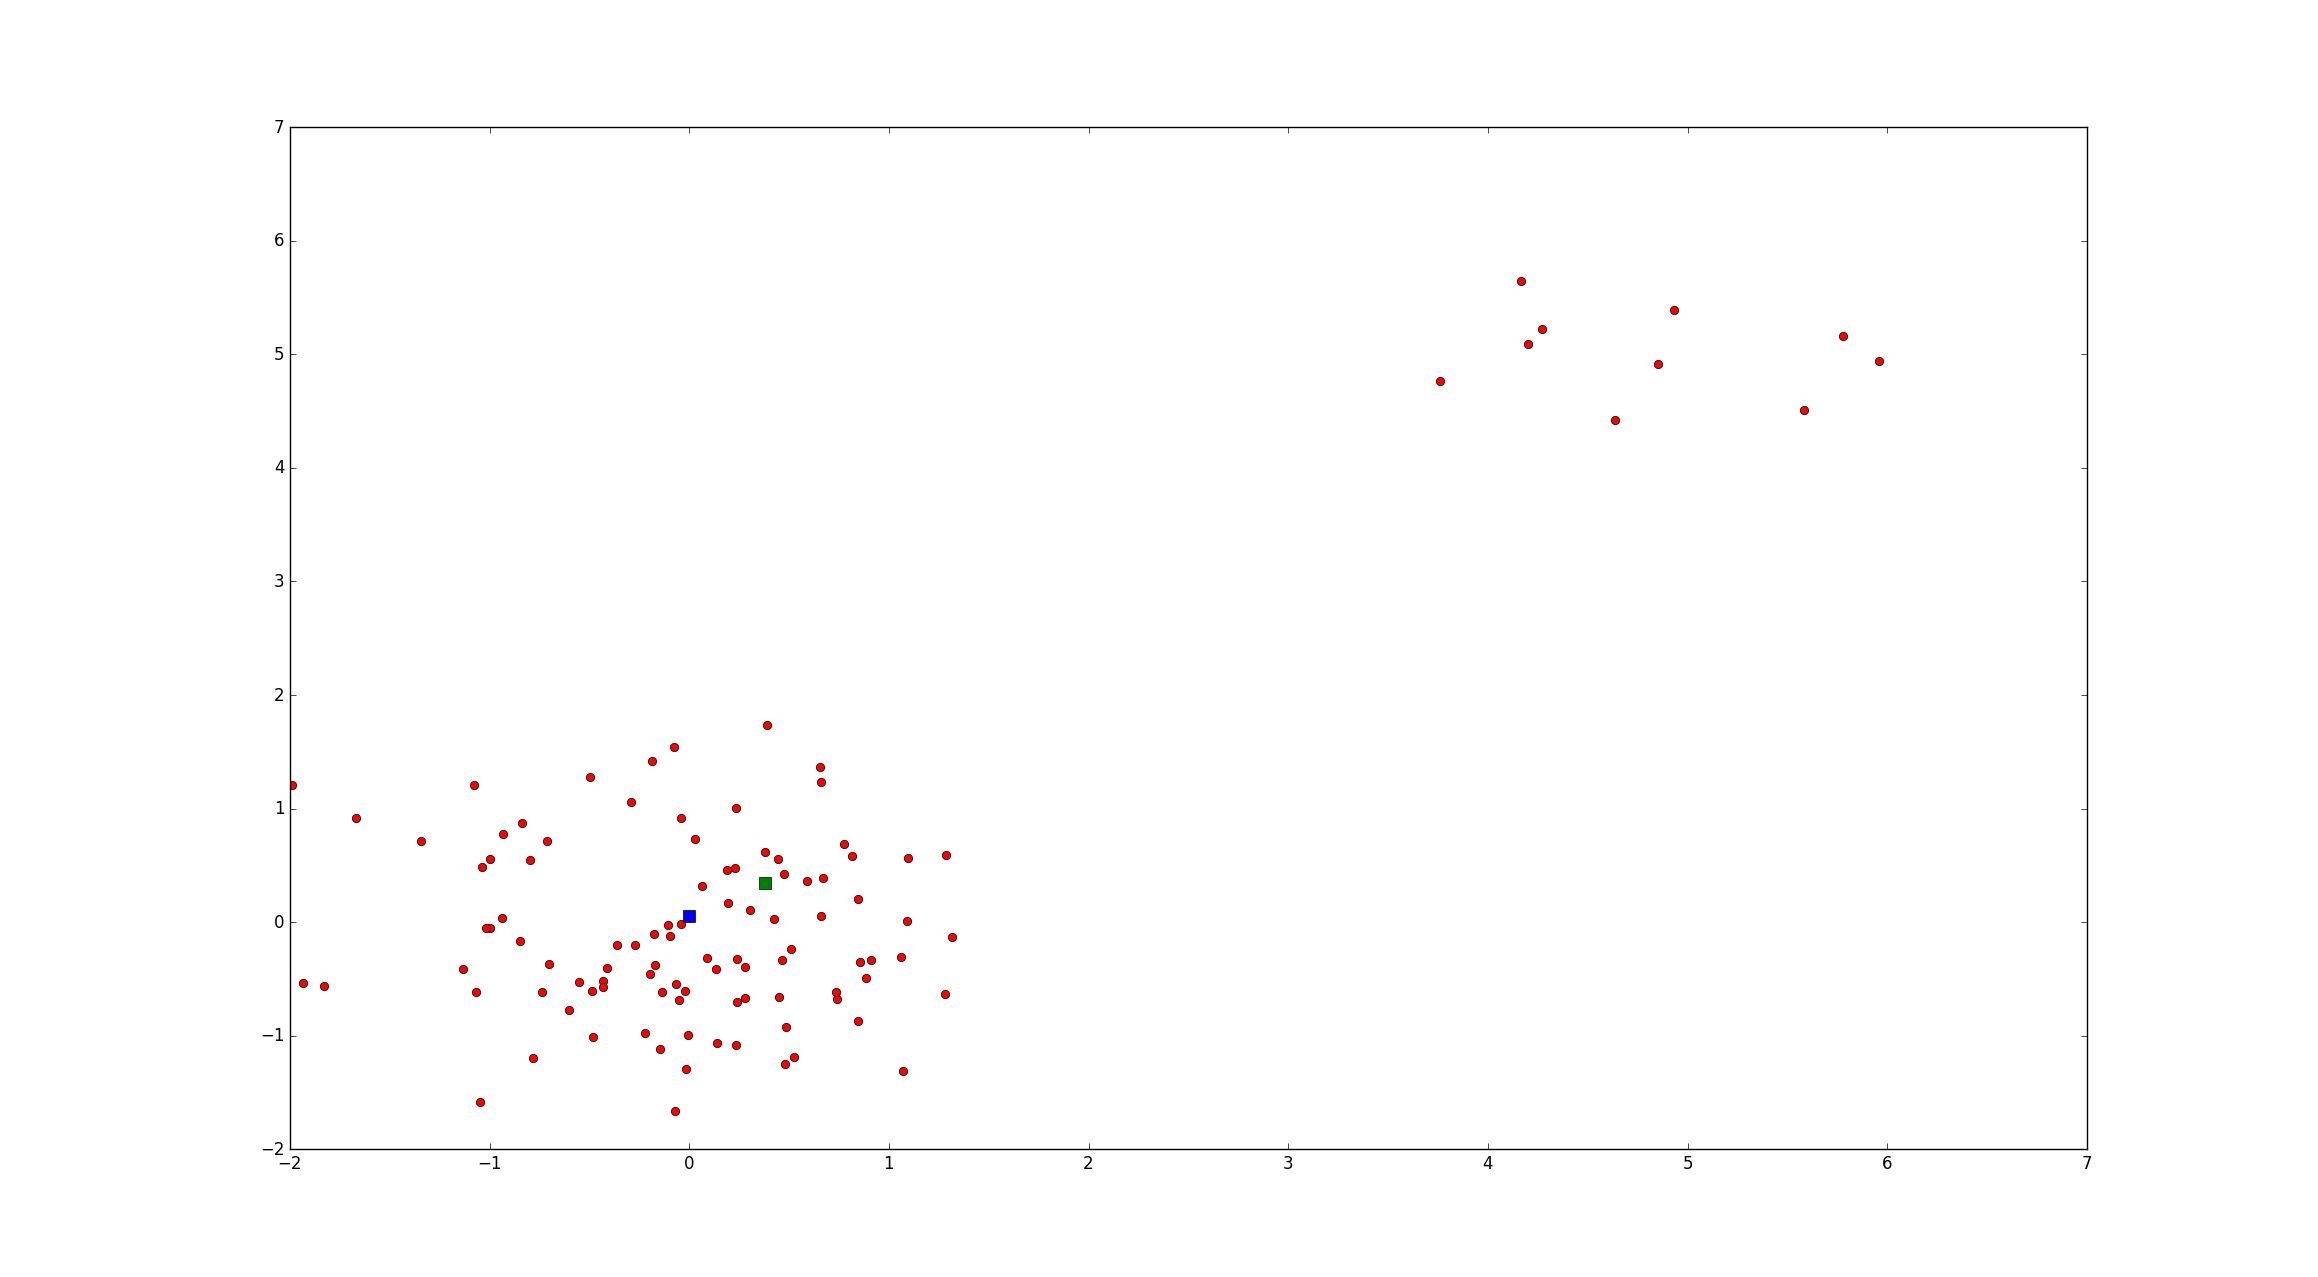
\includegraphics[width=10cm]{GM1.png}
	\end{figure}
\end{frame}

\begin{frame}{Experimento 2}
	Se generaron 100 datos $(x_i, y_i) \sim U(0, 1)$ y se filtraron en una elipse centrada en el origen y con semiejes $(0.9^2, 0.1^2)$ y se añeadieron 5 puntos atípicos de la misma distribución con media $\mu_o = (1, 1)^T$ y matriz de covarianza $\Sigma_o = diag(0.3, 0.3)^T$. Posteriorme se aplicó PCA y PCA robusto con $p = 0.3$.
\end{frame}


\begin{frame}{Experimento 2}
	Resultados obtenidos
	\begin{figure}
		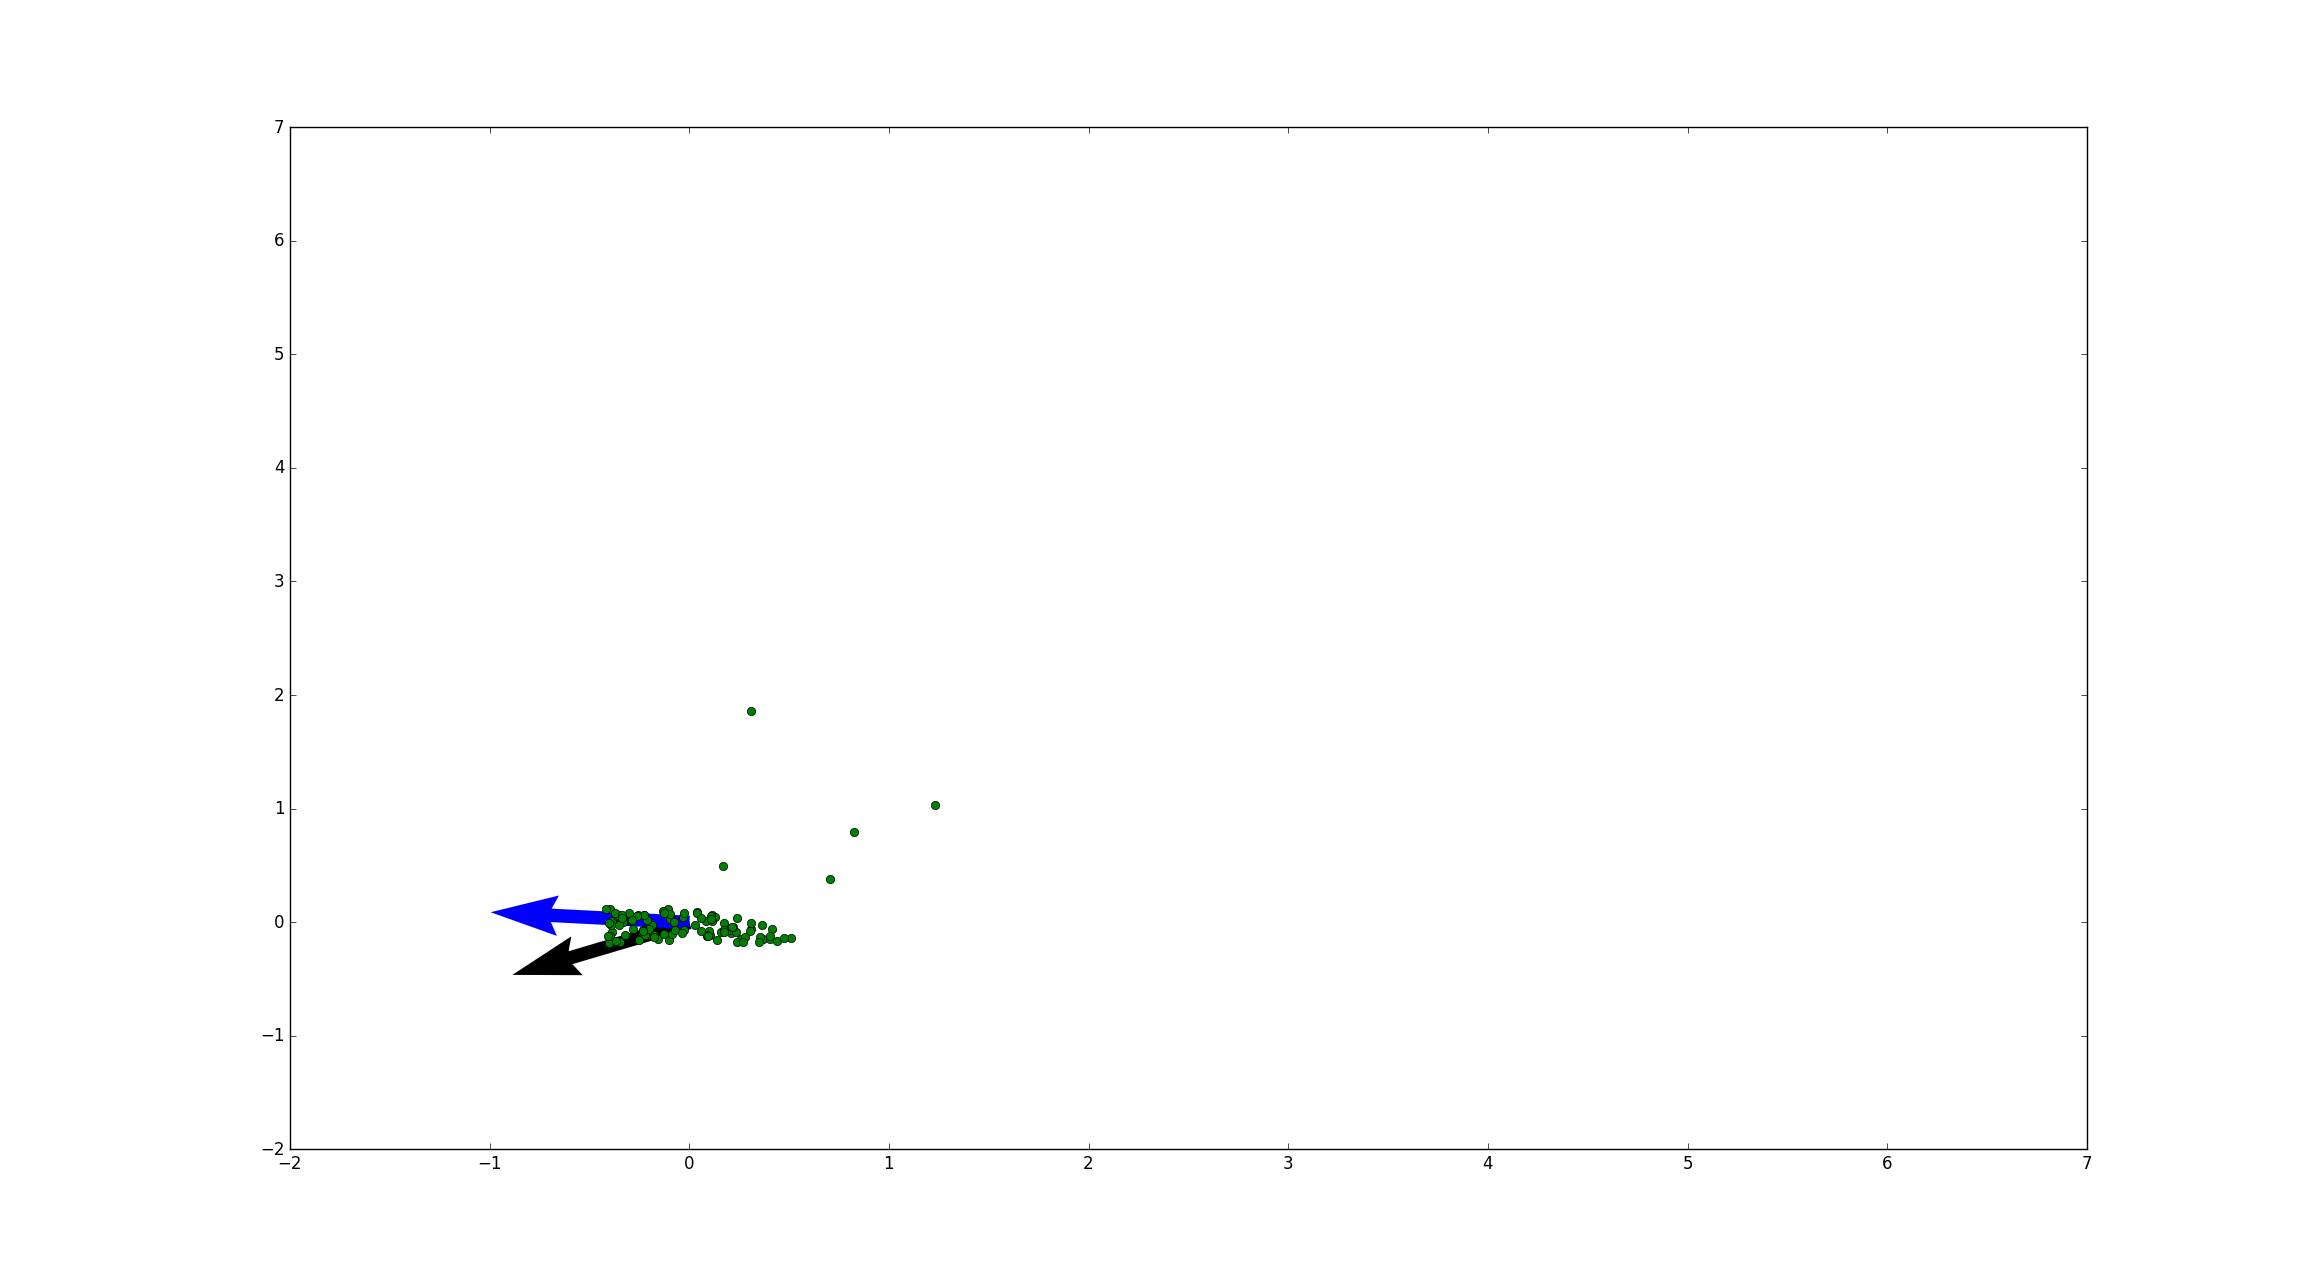
\includegraphics[width=10cm]{GPCA1.png}
	\end{figure}
\end{frame}

\begin{frame}{Experimento 2}
	No todo es bonito $:($
	\begin{figure}
		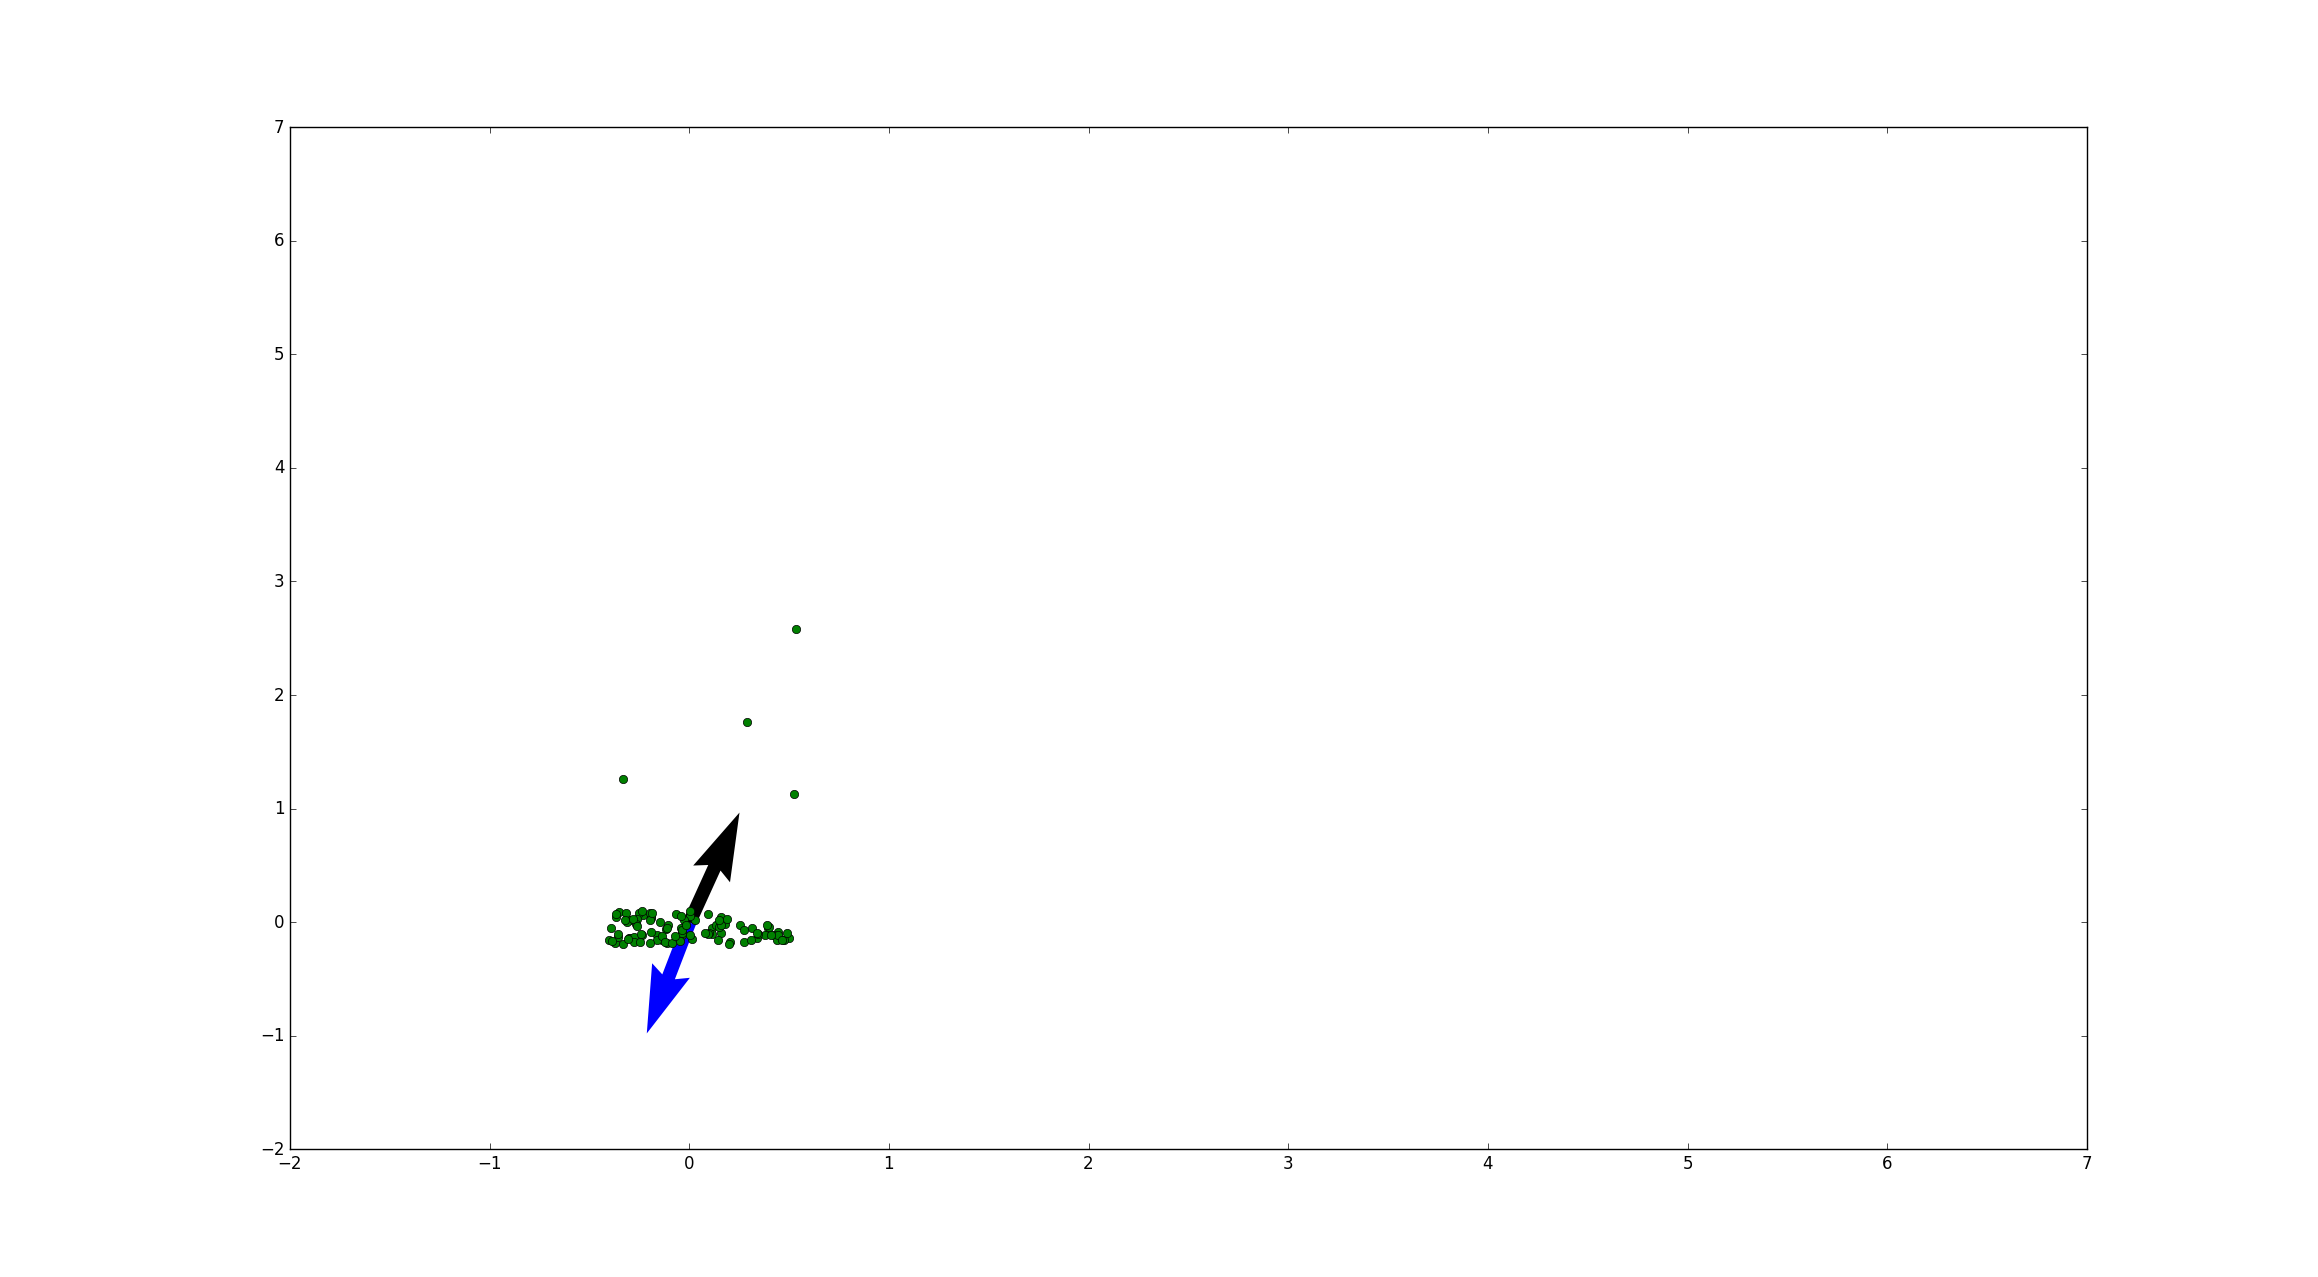
\includegraphics[width=10cm]{GPCA2.png}
	\end{figure}
\end{frame}

\begin{frame}{Experimento 3}
	Se generaron 100 datos usando una distribución univariada Gaussiana $x_i \sim N(0, 1),\ y_i = x_i + \epsilon_i$ con $\epsilon_i \sim N(0, 0.5^2)$ para datos normales y $\epsilon_i \sim N(0, 3^2)$ para datos atípicos. Posteriorme se aplicó PCA y PCA robusto con $p = 0.3$.
\end{frame}


\begin{frame}{Experimento 3}
	Resultados obtenidos
	\begin{figure}
		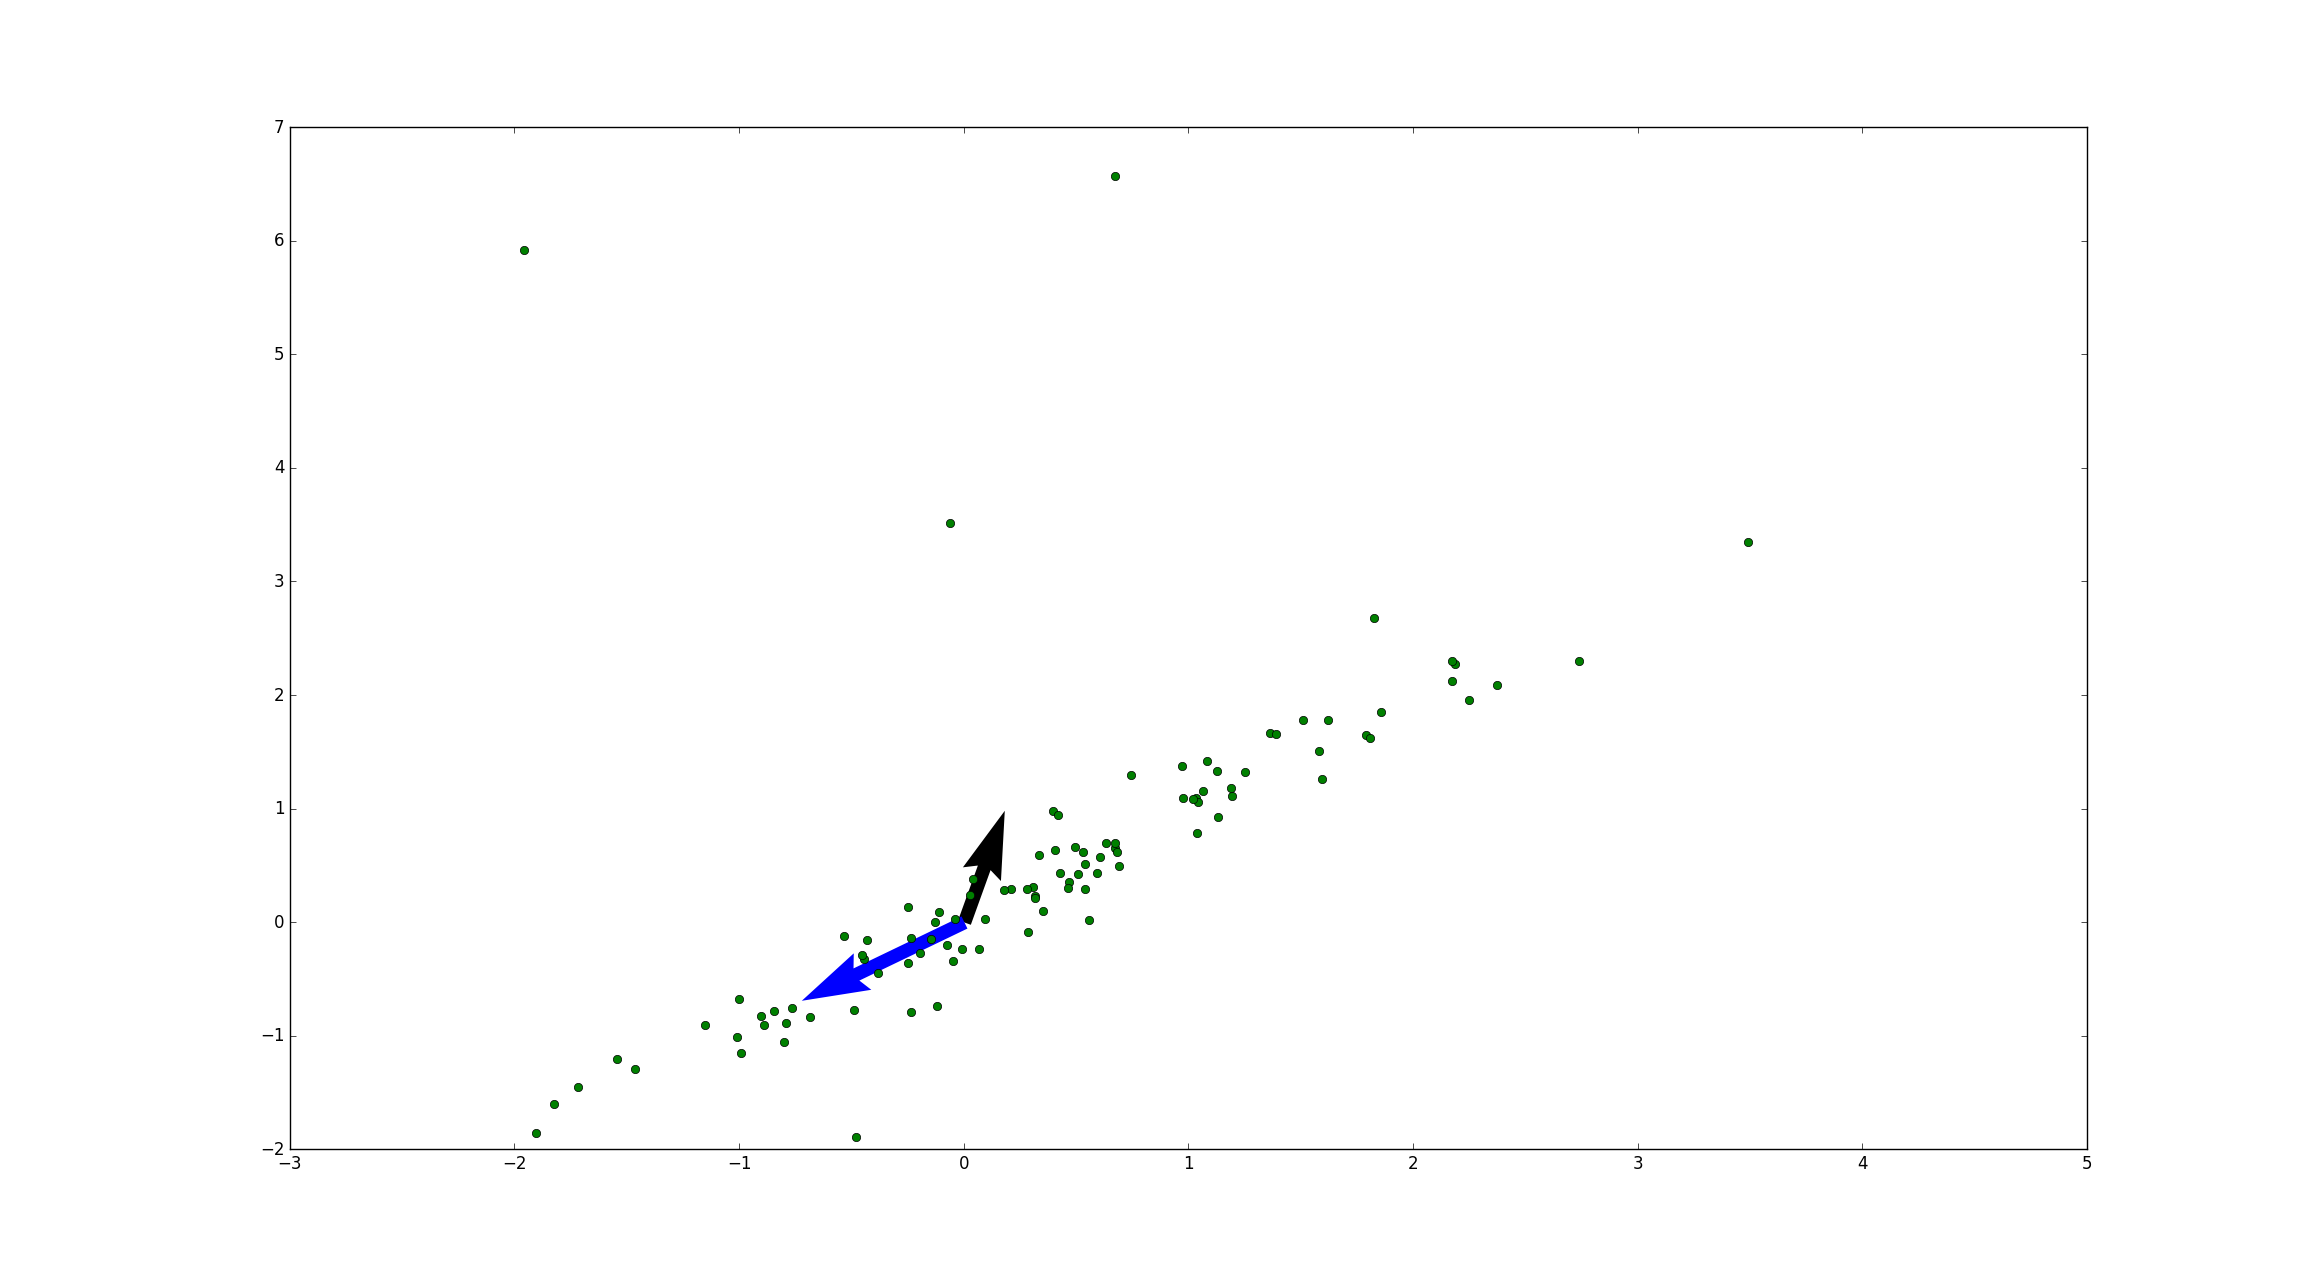
\includegraphics[width=10cm]{GPCA3.png}
	\end{figure}
\end{frame}


\begin{frame}{Experimento 3}
	Gráfica que muestra la relación ángulo - función de costo para ambas versiones de PCA usando el conjunto de datos anterior.
	\begin{figure}
		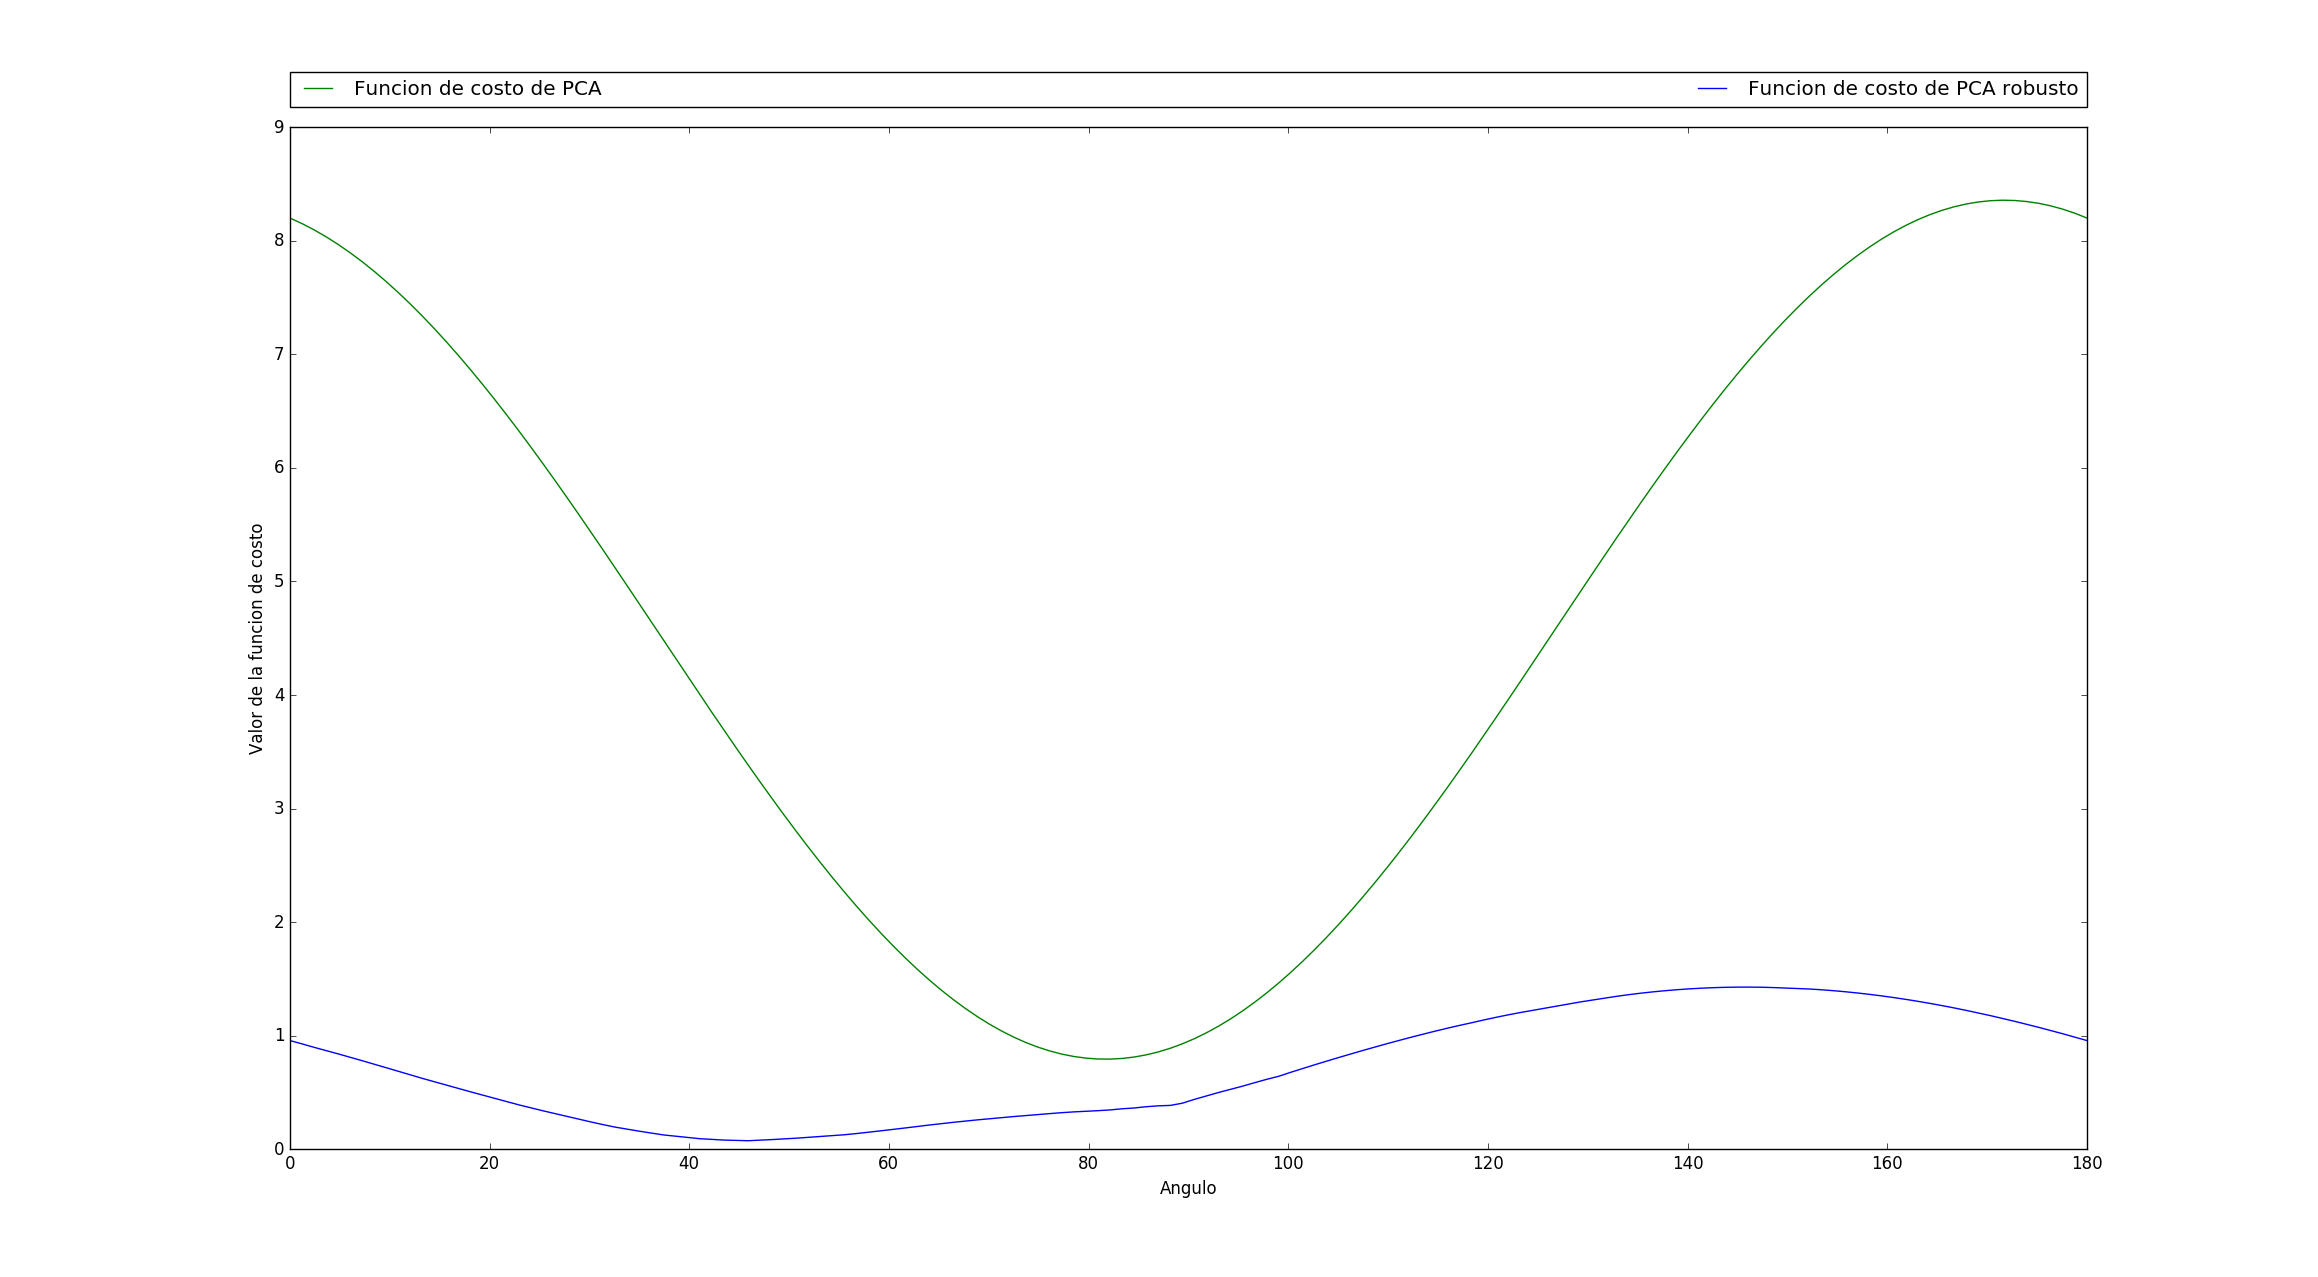
\includegraphics[width=10cm]{CostF.png}
	\end{figure}
\end{frame}

\begin{frame}{Experimento 4}
	Se tomaron 300 muestras del dataset MNIST con los números 3, 8 y 9, luego 60 del mismo dataset con números diferentes para representar datos atípicos. Se normalizaron con norma $L_1$, se hizo reducción de dimension y se aplicó K-Means con 3 clusters.
	\begin{figure}
		
\includegraphics[width=5cm]{MNIST.png}
	\end{figure}
\end{frame}

\begin{frame}{Experimento 4}
	\begin{table}[H]
		\centering
		\caption{Resultados obtenidos del experimento anterior}
		\label{my-label}
		\begin{tabular}{|c|c|c|}
			\hline
			\textbf{m} & \textbf{PCA} & \textbf{PCA-GM} \\ \hline
			50         & 0.26         & 0.37            \\ \hline
			100        & 0.28         & 0.376           \\ \hline
			150        & 0.763        & 0.766           \\ \hline
			200        & 0.76         & 0.766           \\ \hline
			250        & 0.75         & 0.76            \\ \hline
			300        & 0.763        & 0.766           \\ \hline
		\end{tabular}
	\end{table}
\end{frame}

\begin{frame}{Conclusiones}
	\begin{enumerate}
		\item Resultados favorables con respecto a PCA robusto.
		\item Versión robusta en la mayoría de las ecuaciones superior a la versión clásica (al menos en los ejemplos vistos).
		\item La convergencia del algoritmo no está asegurada aunque siempre se logró en los ejemplos probados.
	\end{enumerate}
\end{frame}

\begin{frame}{Referencias}
	\begin{enumerate}
		\item Jiyong Oh, Nojun Kwak. Generalized mean for robust principal component analysis, Pattern Recognition, Elsevier, 2016.
	\end{enumerate}
\end{frame}


\end{document}
